\section{Bundles, connections, and curvature}
\label{sec:connections}
Bundles are simply maps into the universe. By using the extra cellular structure and the even more detailed combinatorial structure of realizations, we can identify inside of HoTT some additional classical definitions.

\subsection{Definitions}
Having the cellular structure allows us to define bundles and connections.
\begin{mydef}
\label{def:connection}
If \( \mm\defeq \mm_0\xrightarrow[]{\imath_0}\cdots\xrightarrow[]{\imath_{n-1}}\mm_n \) is a cellular type and \( f_k:\mm_k\to\uni \) are type families on each skeleton such that all the triangles commute in the diagram:
\end{mydef}
\begin{center}
% https://q.uiver.app/#q=WzAsNixbMCwwLCJcXG1hdGhiYntNfV8wIl0sWzEsMCwiXFxtYXRoYmJ7TX1fMSJdLFsyLDAsIlxcbWF0aGJie019XzIiXSxbNCwwLCJcXG1hdGhiYntNfSJdLFszLDAsIlxcY2RvdHMiXSxbMiwxLCJcXG1hdGhjYWx7VX0iXSxbMCwxLCJcXGltYXRoXzAiXSxbMSwyLCJcXGltYXRoXzEiXSxbMiw0LCJcXGltYXRoXzIiXSxbNCwzLCJcXGltYXRoX3tuLTF9Il0sWzAsNSwiZl8wIl0sWzEsNSwiZl8xIl0sWzIsNSwiZl8yIl0sWzMsNSwiZiIsMl1d
\begin{tikzcd}
  {\mm_0} & {\mm_1} & {\mm_2} & \cdots & {\mm_n} \\
  && {\mathcal{U}}
  \arrow["{\imath_0}", from=1-1, to=1-2]
  \arrow["{f_0}", from=1-1, to=2-3]
  \arrow["{\imath_1}", from=1-2, to=1-3]
  \arrow["{f_1}", from=1-2, to=2-3]
  \arrow["{\imath_2}", from=1-3, to=1-4]
  \arrow["{f_2}", from=1-3, to=2-3]
  \arrow["{\imath_{n-1}}", from=1-4, to=1-5]
  \arrow["f_n"', from=1-5, to=2-3]
\end{tikzcd}
\end{center}
then we say
\begin{itemize}
\item The map \( f_k \) is a \defemph{\( k \)-bundle} on \( \mm \).
\item The pair given by the map \( f_k \) and the proof \( f_k\circ \imath_{k-1}=f_{k-1} \) that \( f_k \) extends \( f_{k-1} \) is called a \defemph{\( k \)-connection on the \( (k-1) \)-bundle \( f_{k-1} \)}.
\end{itemize}


Having the additional structure of a simplicial complex allows us to define curvature, which is a local concept.

\begin{mydef}
If \( \mm \) is the realization of a simplicial complex, such that for each pushout defining \( \mm_k \) we have the diagram
\end{mydef}
\begin{center}
% https://q.uiver.app/#q=WzAsNSxbMCwxLCJcXG1hdGhiYntNfV97ay0xfSJdLFswLDAsIk1fa1xcdGltZXMgXFxwYXJ0aWFsXFxEZWx0YV5rIl0sWzEsMCwiTV9rIl0sWzEsMSwiXFxtYXRoYmJ7TX1fayJdLFsxLDIsIlxcbWF0aGNhbHtVfSJdLFswLDMsIlxcaW1hdGhfe2stMX0iXSxbMSwwLCJcXG1hdGhiYntBfV97ay0xfSIsMl0sWzIsMywiKl97XFxtYXRoYmJ7TX1fa30iXSxbMSwyLCJcXG1hdGhybXtwcn1fMSJdLFszLDEsIiIsMSx7InN0eWxlIjp7Im5hbWUiOiJjb3JuZXItaW52ZXJzZSJ9fV0sWzAsMiwiaF9rIiwwLHsic2hvcnRlbiI6eyJzb3VyY2UiOjQwLCJ0YXJnZXQiOjQwfSwibGV2ZWwiOjJ9XSxbMyw0LCJmX2siXSxbMCw0LCJmX3trLTF9IiwyXSxbMywxMiwiIiwwLHsic2hvcnRlbiI6eyJ0YXJnZXQiOjIwfX1dXQ==
\begin{tikzcd}
  {M_k\times \partial\Delta^k} & {M_k} \\
  {\mathbb{M}_{k-1}} & {\mathbb{M}_k} \\
  & {\mathcal{U}}
  \arrow["{\mathrm{pr}_1}", from=1-1, to=1-2]
  \arrow["{\mathbb{A}_{k-1}}"', from=1-1, to=2-1]
  \arrow["{*_{\mathbb{M}_k}}", from=1-2, to=2-2]
  \arrow["{h_k}", shorten <=10pt, shorten >=10pt, Rightarrow, from=2-1, to=1-2]
  \arrow["{\imath_{k-1}}", from=2-1, to=2-2]
  \arrow[""{name=0, anchor=center, inner sep=0}, "{f_{k-1}}"', from=2-1, to=3-2]
  \arrow["\ulcorner"{anchor=center, pos=0.125, rotate=180}, draw=none, from=2-2, to=1-1]
  \arrow["{f_k}", from=2-2, to=3-2]
  \arrow[shorten >=3pt, Rightarrow, from=2-2, to=0]
\end{tikzcd}
\end{center}

the outer square of which restricts on each face to the diagram

\begin{center}
% https://q.uiver.app/#q=WzAsNCxbMCwxLCJcXG1hdGhiYntNfV97ay0xfSJdLFswLDAsIlxce21fa1xcfVxcdGltZXMgXFxwYXJ0aWFsXFxEZWx0YV5rIl0sWzEsMCwiXFx1bml0Il0sWzEsMSwiXFxtYXRoY2Fse1V9Il0sWzAsM10sWzEsMCwiXFxtYXRoYmJ7QX1fe2stMX0iLDJdLFsyLDMsIipfe1xcbWF0aGJie019X2t9Il0sWzEsMiwiISJdLFswLDIsIlxcZmxhdF9rIiwwLHsic2hvcnRlbiI6eyJzb3VyY2UiOjQwLCJ0YXJnZXQiOjQwfSwibGV2ZWwiOjJ9XV0=
\begin{tikzcd}
  {\{m_k\}\times \partial\Delta^k} & \unit \\
  {\mathbb{M}_{k-1}} & {\mathcal{U}}
  \arrow["{!}", from=1-1, to=1-2]
  \arrow["{\mathbb{A}_{k-1}}"', from=1-1, to=2-1]
  \arrow["{*_{\mathbb{M}_k}}", from=1-2, to=2-2]
  \arrow["{\flat_k}", shorten <=11pt, shorten >=11pt, Rightarrow, from=1-2, to=2-1]
  \arrow[from=2-1, to=2-2]
\end{tikzcd}
\end{center}
then we say the filler \( \flat_k \) is called a \defemph{flatness structure for the face \( m_k \)}, and its ending path is called \defemph{curvature at the face \( m_k \)}.

Although all the pushout diagrams are introducing hub points for each edge and face, in practice we will ignore those. But in the case of flatness, which we will use extensively, we should clarify what its type is when we are ignoring hubs. If we have a face \( F \) with vertices \( v_1, v_2, v_3 \) and paths \( e_{ij}:v_i=v_j \) that are realizations of edges, and the loop \( \ell_F\defeq e_{12}\cdot e_{23}\cdot e_{31}\) then we will write \(\flat(\ell_F):\id_{f_0(v_1)}=f_1(\ell_F)\) for a 2-path filling this loop.

The definitions can be digested to give
\begin{mylemma}
\label{lem:extend_faces}
Given \( f_{k-1} \) as above, a \( k \)-connection exists if and only if there exists a flatness structure for each \( k \)-face.
\end{mylemma}

On a 2-dimensional cellular type \( \mm\defeq\mm_0\to\mm_1\to\mm_2 \) the terminology works out as follows: a 0-bundle on \( \mm \) is a map \( T_0:\mm_0\to\uni \). A 1-connection on \( T_0 \) is an extension \( T_1:\mm_1\to\uni \). A 2-connection on \( T_1 \) is an extension \( T_2:\mm_2\to\uni \). Classically, a 1-extension that extends to a 2-connection is called \emph{flat}.

\subsection{Flat connections as local trivializations}
\label{sec:localtriv}
This section can be viewed as an extended remark. The observation we want to make is that the data of a 2-bundle on a realization of a 2-dimensional simplicial complex is related to the construction of local trivializations: the fiber at one vertex can be extended throughout a single face coherently, using the connection (the extension of the classifying map to the edges) to specify isomorphisms with the fibers at the other points, and the higher connections to establish commutativity between these. 

We introduce a notation more suitable for the algebra of charts and overlaps: denote the fiber at \( v_i \) by \( T_i \) and denote transport along \( e_{ij}:v_i=v_j \) by \( T_{ji}:T_i\to T_j \). The indices are ordered from right to left, which is compatible with function composition notation. Denote the inverse function by swapping indices: \( T_{ij}\defeq T_{ji}^{-1} \). Assume we have some fixed isomorphism \( T_i=S^1 \), and to avoid composing everything with this function we will assume it is \( \id \). In the diagram below we see the data arranged so that our bundles fibers are on the left, and the fiber of a trivial bundle is on the right.
\begin{center}
% https://q.uiver.app/#q=WzAsNixbMCwwLCJUX2kiXSxbMCwxLCJUX2oiXSxbMCwyLCJUX2siXSxbMSwwLCJTXjEiXSxbMSwxLCJTXjEiXSxbMSwyLCJTXjEiXSxbMCwzLCJcXG1hdGhybXtpZH0iLDAseyJsZXZlbCI6Miwic3R5bGUiOnsiaGVhZCI6eyJuYW1lIjoibm9uZSJ9fX1dLFswLDEsIlRfe2ppfSIsMl0sWzEsMiwiVF97a2p9IiwyXSxbMSw0LCJUX3tpan0iLDJdLFsyLDUsIlRfe2lqfVRfe2prfSIsMl0sWzMsNCwiIiwwLHsibGV2ZWwiOjIsInN0eWxlIjp7ImhlYWQiOnsibmFtZSI6Im5vbmUifX19XSxbNCw1LCIiLDAseyJsZXZlbCI6Miwic3R5bGUiOnsiaGVhZCI6eyJuYW1lIjoibm9uZSJ9fX1dLFswLDIsIlRfe2tpfSIsMix7ImN1cnZlIjo1fV0sWzMsNSwiIiwxLHsiY3VydmUiOi01LCJsZXZlbCI6Miwic3R5bGUiOnsiaGVhZCI6eyJuYW1lIjoibm9uZSJ9fX1dLFsxLDEzLCJcXGZsYXRfe2lqa30iLDIseyJzaG9ydGVuIjp7InRhcmdldCI6MjB9fV1d
\begin{tikzcd}
  {T_i} & {S^1} \\
  {T_j} & {S^1} \\
  {T_k} & {S^1}
  \arrow["{\mathrm{id}}", equals, from=1-1, to=1-2]
  \arrow["{T_{ji}}"', from=1-1, to=2-1]
  \arrow[""{name=0, anchor=center, inner sep=0}, "{T_{ki}}"', curve={height=40pt}, from=1-1, to=3-1]
  \arrow[equals, from=1-2, to=2-2]
  \arrow[curve={height=-40pt}, equals, from=1-2, to=3-2]
  \arrow["{T_{ij}}"', from=2-1, to=2-2]
  \arrow["{T_{kj}}"', from=2-1, to=3-1]
  \arrow[equals, from=2-2, to=3-2]
  \arrow["{T_{ij}T_{jk}}"', from=3-1, to=3-2]
  \arrow["{\flat_{ijk}}"', shorten >=4pt, Rightarrow, from=2-1, to=0]
\end{tikzcd}
\end{center}
The two middle squares commute definitionally. Call these two squares together the back face. The left triangle is filled by the flatness structure on the face, and the right triangular filler is trivial. There is also a filler needed for the front, i.e. the outer square. This requires proving that \( T_{ki}T_{ij}T_{jk}=\id \), which is supplied by the flatness structure. There is also a 3-cell filling the interior of this prism, mapping the back face plus the left triangle filler to the front face plus the right triangle filler. These two faces both consist of one or two identities concatenated with the flatness structure, and so the 3-cell is definitional.

This relationship between flatness structure and local triviality of a chart can be compared to the classical result that on a paracompact, simply connected manifold (such as a single chart), a connection on a principal bundle is flat if and only if the bundle is trivial. See for example \cite{kobayashinomizu} Corollary 9.2.

\subsection{The tangent bundle of the sphere}
We will build up a map \( T \) out of \( \oo_0\to\oo_1\to\oo \) which is meant to be a model of the tangent bundle of the sphere. The link function will serve as our approximation to the tangent space. Taking the link of a vertex gives us a map from vertices to polygons, so the codomain is \( \EMzo \).

If \( \{b, r, g, o\} \) are four vertices in \( \oo \), the notation \( \hgr{brgo} \) refers to the 4-gon spanned by these four vertices and the edges of \( \oo \) that connect them to each other.

\begin{mydef}
\( T_0\defeq\link:\oo_0\to\EMzo \) is given by:
\begin{align*}
\link(w) &= \hgr{brgo} & \link(r) &= \hgr{wbyg} \\
\link(y) &= \hgr{bogr} & \link(g) &= \hgr{wryo} \\
\link(b) &= \hgr{woyr} & \link(o) &= \hgr{wgyb}
\end{align*}

We chose these orderings for the vertices in the link, by visualizing standing at the given vertex as if it were the north pole, then looking south and enumerating the link in clockwise order, starting from \( w \) if possible, else \( b \).
\end{mydef}

\begin{figure}[h]
\centering
\begin{figure}[h]
\centering
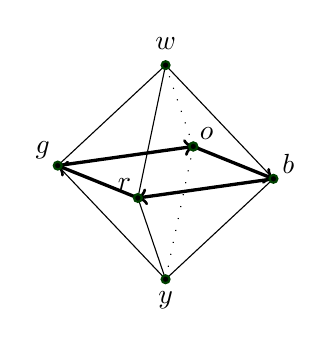
\begin{tikzpicture}%
  [x={(-0.860769cm, -0.121512cm)},
  y={(0.508996cm, -0.205391cm)},
  z={(-0.000053cm, 0.971107cm)},
  scale=1,
  eqback/.style={->, very thick},
  back/.style={loosely dotted, thin},
  eqedge/.style={->, very thick},
  edge/.style={black, thin},
  facet/.style={fill=blue!95!black,fill opacity=0.0},
  vertex/.style={inner sep=1pt,circle,draw=green!25!black,fill=black,thick}]
\coordinate (-1, -1, 0) at (-1, -1, 0);
\coordinate (-1, 1, 0) at (-1, 1, 0);
\coordinate (0, 0, -1) at (0, 0, -1);
\coordinate (0, 0, 1) at (0, 0, 1);
\coordinate (1, -1, 0) at (1, -1, 0);
\coordinate (1, 1, 0) at (1, 1, 0);
%% Drawing edges in the back
%%
\draw[edge,eqback] (-1, -1, 0) -- (-1, 1, 0);
\draw[edge,back] (-1, -1, 0) -- (0, 0, -1.4);
\draw[edge,back] (-1, -1, 0) -- (0, 0, 1.4);
\draw[edge,eqback] (1, -1, 0) -- (-1, -1, 0);
%% Drawing vertices in the back
%%
\node[vertex] at (-1, -1, 0)     {};
%% Drawing the facets
%%
\fill[facet] (1, 1, 0) -- (0, 0, -1.4) -- (1, -1, 0) -- cycle {};
\fill[facet] (1, 1, 0) -- (0, 0, 1.4) -- (1, -1, 0) -- cycle {};
\fill[facet] (1, 1, 0) -- (-1, 1, 0) -- (0, 0, 1.4) -- cycle {};
\fill[facet] (1, 1, 0) -- (-1, 1, 0) -- (0, 0, -1.4) -- cycle {};
%% Drawing edges in the front
%%
\draw[edge] (-1, 1, 0) -- (0, 0, -1.4);
\draw[edge] (-1, 1, 0) -- (0, 0, 1.4);
\draw[eqedge] (-1, 1, 0) -- (1, 1, 0);
\draw[edge] (0, 0, -1.4) -- (1, -1, 0);
\draw[edge] (0, 0, -1.4) -- (1, 1, 0);
\draw[edge] (0, 0, 1.4) -- (1, -1, 0);
\draw[edge] (0, 0, 1.4) -- (1, 1, 0);
\draw[eqedge] (1, 1, 0) -- (1, -1, 0);
%% Drawing the vertices in the front
%%
\begin{scope}[nodes=vertex]
\node[label=above right:\( b \)] at (-1, 1, 0)     {};
\node[label=below:\( y \)] at (0, 0, -1.4)     {};
\node[label=above:\( w \)] at (0, 0, 1.4)     {};
\node[label=above left:\( g \)] at (1, -1, 0)     {};
\node[label=above left:\( r \)] at (1, 1, 0)     {};
\node[label=above right:\( o \)] at (-1, -1, 0)     {};
\end{scope}
\end{tikzpicture}

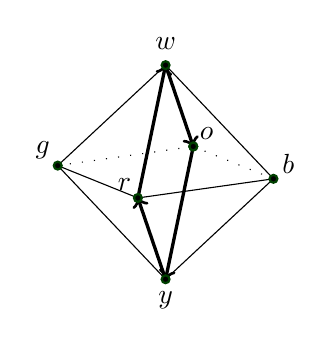
\begin{tikzpicture}%
  [x={(-0.860769cm, -0.121512cm)},
  y={(0.508996cm, -0.205391cm)},
  z={(-0.000053cm, 0.971107cm)},
  scale=1,
  eqback/.style={->, very thick},
  back/.style={loosely dotted, thin},
  eqedge/.style={->, very thick},
  edge/.style={black, thin},
  facet/.style={fill=blue!95!black,fill opacity=0.0},
  vertex/.style={inner sep=1pt,circle,draw=green!25!black,fill=black,thick}]
\coordinate (-1, -1, 0) at (-1, -1, 0);
\coordinate (-1, 1, 0) at (-1, 1, 0);
\coordinate (0, 0, -1) at (0, 0, -1);
\coordinate (0, 0, 1) at (0, 0, 1);
\coordinate (1, -1, 0) at (1, -1, 0);
\coordinate (1, 1, 0) at (1, 1, 0);
%% Drawing edges in the back
%%
\draw[edge,back] (-1, -1, 0) -- (-1, 1, 0);
\draw[edge,eqback] (-1, -1, 0) -- (0, 0, -1.4);
\draw[edge,eqback] (0, 0, 1.4) -- (-1, -1, 0);
\draw[edge,back] (1, -1, 0) -- (-1, -1, 0);
%% Drawing vertices in the back
%%
\node[vertex] at (-1, -1, 0)     {};
%% Drawing the facets
%%
\fill[facet] (1, 1, 0) -- (0, 0, -1.4) -- (1, -1, 0) -- cycle {};
\fill[facet] (1, 1, 0) -- (0, 0, 1.4) -- (1, -1, 0) -- cycle {};
\fill[facet] (1, 1, 0) -- (-1, 1, 0) -- (0, 0, 1.4) -- cycle {};
\fill[facet] (1, 1, 0) -- (-1, 1, 0) -- (0, 0, -1.4) -- cycle {};
%% Drawing edges in the front
%%
\draw[edge] (-1, 1, 0) -- (0, 0, -1.4);
\draw[edge] (-1, 1, 0) -- (0, 0, 1.4);
\draw[edge] (-1, 1, 0) -- (1, 1, 0);
\draw[edge] (0, 0, -1.4) -- (1, -1, 0);
\draw[eqedge] (0, 0, -1.4) -- (1, 1, 0);
\draw[edge] (0, 0, 1.4) -- (1, -1, 0);
\draw[eqedge] (1, 1, 0) -- (0, 0, 1.4) ;
\draw[edge] (1, 1, 0) -- (1, -1, 0);
%% Drawing the vertices in the front
%%
\begin{scope}[nodes=vertex]
\node[label=above right:\( b \)] at (-1, 1, 0)     {};
\node[label=below:\( y \)] at (0, 0, -1.4)     {};
\node[label=above:\( w \)] at (0, 0, 1.4)     {};
\node[label=above left:\( g \)] at (1, -1, 0)     {};
\node[label=above left:\( r \)] at (1, 1, 0)     {};
\node[label=above right:\( o \)] at (-1, -1, 0)     {};
\end{scope}
\end{tikzpicture}

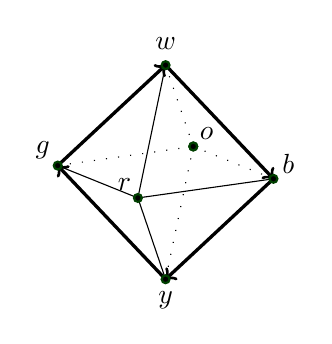
\begin{tikzpicture}%
  [x={(-0.860769cm, -0.121512cm)},
  y={(0.508996cm, -0.205391cm)},
  z={(-0.000053cm, 0.971107cm)},
  scale=1,
  eqback/.style={->, very thick},
  back/.style={loosely dotted, thin},
  eqedge/.style={->, very thick},
  edge/.style={black, thin},
  facet/.style={fill=blue!95!black,fill opacity=0.0},
  vertex/.style={inner sep=1pt,circle,draw=green!25!black,fill=black,thick}]
\coordinate (-1, -1, 0) at (-1, -1, 0);
\coordinate (-1, 1, 0) at (-1, 1, 0);
\coordinate (0, 0, -1) at (0, 0, -1);
\coordinate (0, 0, 1) at (0, 0, 1);
\coordinate (1, -1, 0) at (1, -1, 0);
\coordinate (1, 1, 0) at (1, 1, 0);
%% Drawing edges in the back
%%
\draw[edge,back] (-1, -1, 0) -- (-1, 1, 0);
\draw[edge,back] (-1, -1, 0) -- (0, 0, -1.4);
\draw[edge,back] (-1, -1, 0) -- (0, 0, 1.4);
\draw[edge,back] (1, -1, 0) -- (-1, -1, 0);
%% Drawing vertices in the back
%%
\node[vertex] at (-1, -1, 0)     {};
%% Drawing the facets
%%
\fill[facet] (1, 1, 0) -- (0, 0, -1.4) -- (1, -1, 0) -- cycle {};
\fill[facet] (1, 1, 0) -- (0, 0, 1.4) -- (1, -1, 0) -- cycle {};
\fill[facet] (1, 1, 0) -- (-1, 1, 0) -- (0, 0, 1.4) -- cycle {};
\fill[facet] (1, 1, 0) -- (-1, 1, 0) -- (0, 0, -1.4) -- cycle {};
%% Drawing edges in the front
%%
\draw[eqedge] (-1, 1, 0) -- (0, 0, -1.4);
\draw[eqedge] (0, 0, 1.4) -- (-1, 1, 0);
\draw[edge] (-1, 1, 0) -- (1, 1, 0);
\draw[eqedge] (0, 0, -1.4) -- (1, -1, 0);
\draw[edge] (0, 0, -1.4) -- (1, 1, 0);
\draw[eqedge] (1, -1, 0) -- (0, 0, 1.4);
\draw[edge] (0, 0, 1.4) -- (1, 1, 0);
\draw[edge] (1, 1, 0) -- (1, -1, 0);
%% Drawing the vertices in the front
%%
\begin{scope}[nodes=vertex]
\node[label=above right:\( b \)] at (-1, 1, 0)     {};
\node[label=below:\( y \)] at (0, 0, -1.4)     {};
\node[label=above:\( w \)] at (0, 0, 1.4)     {};
\node[label=above left:\( g \)] at (1, -1, 0)     {};
\node[label=above left:\( r \)] at (1, 1, 0)     {};
\node[label=above right:\( o \)] at (-1, -1, 0)     {};
\end{scope}
\end{tikzpicture}
\caption{The equators for \( w, b, r \).}
\end{figure}
\caption{\( \link \) for the vertices \( w, b\) and \( r \).}
\label{fig:triangle_of_equators}
\end{figure}

To extend \( T_0 \) to a function \( T_1 \) on the 1-skeleton we have some freedom. We will do something motivated by the figures we have been drawing of an octahedron embedded in 3-dimensional space. We will imagine how \( T_1 \) changes as we slide from point to point in the embedding shown in the figures. Sliding from \( w \) to \( b \) and tipping the link as we go, we see \( r\mapsto r \) and \( o\mapsto o \) because those lie on the axis of rotation. Then \( g\mapsto w \) and \( b\mapsto y \). 


\begin{mydef}
Define \( T_1:\oo_1\to\EMzo \) on just the 1-skeleton by extending \( T_0 \) as follows:
Transport away from \( w \):
\begin{itemize}
\item \( T_1(wr):\hgr{brgo}\mapsto \hgr{bygw} \) (\( b, g \) fixed)
\item \( T_1(wg):\hgr{brgo}\mapsto \hgr{wryo} \)
\item \( T_1(wb):\hgr{brgo}\mapsto \hgr{yrwo} \) (\( r, o \) fixed)
\item \( T_1(wo):\hgr{brgo}\mapsto \hgr{bwgy} \)
\end{itemize}
Transport away from \( y \):
\begin{itemize}
\item \( T_1(yb):\hgr{bogr}\mapsto \hgr{woyr} \)
\item \( T_1(yr):\hgr{bogr}\mapsto \hgr{bygw} \)
\item \( T_1(yg):\hgr{bogr}\mapsto \hgr{yowr} \)
\item \( T_1(yo):\hgr{bogr}\mapsto \hgr{bwgy} \)
\end{itemize}
Transport along the equator:
\begin{itemize}
\item \( T_1(br):\hgr{woyr}\mapsto \hgr{wbyg} \) 
\item \( T_1(rg):\hgr{wbyg}\mapsto \hgr{wryo} \)
\item \( T_1(go):\hgr{wryo}\mapsto \hgr{wgyb} \)
\item \( T_1(ob):\hgr{wgyb}\mapsto \hgr{woyr} \)
\end{itemize}
\label{def:transport_oo}
\end{mydef}

It's very important to be able to visualize what \( T_1 \) does to triangular paths such as \( wb\cdot br\cdot rw \) (which circulates around the boundary of face \( wbr \)). You can see it if you imagine Figure~\ref{fig:triangle_of_equators} as the frames of a short movie. Or you can place your palm over the top of a cube and note where your fingers are pointing, then slide your hand to an equatorial face, then along the equator, then back to the top. The answer is: you come back rotated clockwise by a quarter-turn, which we saw in Definition~\ref{def:rotation} where it is called \( \hgr{R} \).

Now let's extend \( T_1 \) to all of \( \oo \) by providing values for the eight faces. The face \( wbr \) is a path from \( \refl_w \) to the concatenation \( wb\cdot br\cdot rw \), and so the image of \( wbr \) under the extended version of \( T_1 \) must be a homotopy from \( \refl_{T_1(w)} \) to \( T_1(wb\cdot br\cdot rw) \). Here \emph{there is no additional freedom}.

\begin{mydef}
\label{def:octahedron_curvature}
Define \( T_2:\oo\to\EMzo \) by extending \( T_1 \) to the faces as follows (making use of \( H_R \) from Lemma~\ref{lem:rotation}):
\begin{multicols}{2}
\begin{itemize}
\item \( T_2(wbr)=H_R \) 
\item \( T_2(wrg)=H_R \)
\item \( T_2(wgo)=H_R \)
\item \( T_2(ybo)=H_R \)
\item \( T_2(yrb)=H_R \) 
\item \( T_2(ygr)=H_R \)
\item \( T_2(yog)=H_R \)
\item \( T_2(ybo)=H_R \)
\end{itemize}
\end{multicols}
Defining these flatness structures suffices to define \( T_2 \) by Lemma~\ref{lem:extend_faces}.
\end{mydef}

\subsection{Existence of connections}
\label{sec:existence}
How confident can we be that we can always define a connection on the realization of an arbitrary simplicial complex? Two things make the octahedron example special: the link is a 4-gon at every vertex (as opposed to having a variable number of vertices), and every transport map extends to a rotation of the entire octahedron in 3-dimensional space. This imposed a coherence on the interactions of all the choices we made for the connection, which we can worry may not exist for more complex combinatorial data.

We know as a fact outside of HoTT that any combinatorial surface that has been realized as a triangulated surface embedded in 3-dimensional euclidean space can inherit the parallel transport entailed in the embedding. We could then approximate that data to arbitrary precision with enough subdivision of the fibers of \( T \).

What would a proof inside of HoTT look like? We will leave this as an open question.

